\chapter{从传统虚拟化到虚拟容器}
\label{cha:virtualization-and-container}

虚拟化技术从 2008 开始越来越热,到了今天,已经成为了企业 IT 技术中必不可少的了。
本章节首先介绍虚拟化技术的演变以及在发展过程中产生的几种类型,然后介绍几种用户
层 (user-land) 的虚拟化管理工具,然后介绍本次实验采用的宿主系统 CentOS 7 的
一些特性,最后罗列 OpenStack 支持的几种虚拟化方案。

在下文中,如果没有特殊说明,用虚拟机管理程序指代 hypervisor ,用宿主机
指代 host ,也就是承载虚拟机管理程序的物理机器和上面运行的操作系统,用
客户机或者客户虚拟机指代 guest ,也就是运行在宿主机上由虚拟机管理程序
模拟出的环境上的宾客操作系统及相关软件。

\section{虚拟化技术的演变}

和其它大多数技术一样,虚拟化技术也不是一蹴而就的,它经历了以下几种形态的演变和发展
~\cite{deep-into-kvm}:

\subsection{软件模拟}
\label{emulators}

严格来说,模拟器 (emulator) 不是一种虚拟化方式,但是它也可以实现在宿主机上
运行不同的客户机操作系统。它的出现早于虚拟化技术,而且实现的方式形形色色,例如
早期的 Macintosh 电脑可以安装兼容 DOS 系统的扩展卡,从而运行为 PC 编写的
程序。现在常见的形式是软件模拟,例如 QEMU \footnote{QEMU 可以和 KVM 配合,
工作在 virtualizer 模式,在这里只讨论 emulator 模式}。

\begin{figure}[h]
    \centering
    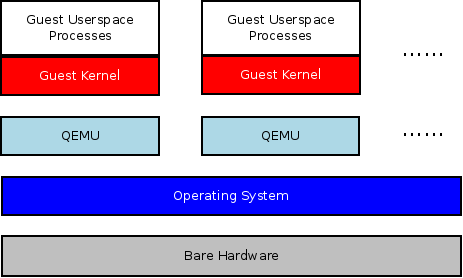
\includegraphics[width=0.7\textwidth]{qemu-arch}
    \caption{QEMU 的基本结构}
\end{figure}

和 Bochs 不同,QEMU 不仅能模拟 X86 架构的处理器,还能支持 ARM / MIPS / PowerPC
 / Sparc / Xtensa 等多种架构的处理器~\cite{qemu-internals}。
而且 QEMU 和 Valgrind 一样使用的是动态翻译。所谓静态翻译,就是不需要执行程序本身,
一次读入整个二进制文件,完成翻译;所谓动态翻译,就是在执行过程中只看一小段程序,
比如一个基本块 (basic block) ,然后翻译并缓存 (caching)翻译好的目标代码。
这样的好处是二进制程序只在需要的时候被翻译,比如一个循环,执行一次之后
又跳转回到和一开始相同的代码,那么只需要指向缓存中已经翻译好的代码就可以了,
而不用重新翻译一遍。

当然 Valgrind 本质上是一个检查内存错误的 memcheck 工具,这是它和 QEMU 根本上的不同。
如果模拟器工作在纯软件模拟,执行效率是不高的,但是好处是理论上可以模拟任何硬件,
以至于不存在的硬件。

\subsection{虚拟化层翻译}

\subsubsection{软件全虚拟化}
\label{subsubsec:software-virt}

成立于 1998 年的 VMWare 最早提出了软件虚拟化的概念。和~\ref{emulators}小节提到的
模拟器不同,VMWare 的虚拟机管理程序不需要模拟物理上并不存在的硬件的指令集系统,既不像
静态翻译一样需要一个接一个地把程序的 CPU 指令翻译成宿主机上的指令,也不像动态翻译一样
需要在基本块第一次运行的时候翻译整段代码。但是 VMWare 需要虚拟各种硬件适配器,例如
网络适配器、图形适配器或者磁盘。

VMWare 的出现远早于 Intel 或是 AMD 的硬件虚拟化扩展 (Intel VT 或是 AMD-V),
那么最初的 VMWare 是怎么靠纯软件的方法实现虚拟机管理程序的呢?
本科操作系统课讲过,X86 处理器的指令划分为 4 个特权级,
也就是 Ring 0 、Ring 1 、Ring 2 和 Ring 3 。操作系统和一些设备驱动的特权级最高,
一般使用 Ring 0 ,用户态 (user-mode) 程序特权级比较低,一般使用 Ring 3 。
Ring 1 和 Ring 2 很少使用\footnote{当然,这取决于操作系统内核的设计,比如
OS/2 使用三个 Ring —— 内核和驱动使用 Ring 0,可以访问 I/O 的特权程序使用
Ring 2 ,普通用户态程序使用 Ring 3;OpenVMS 使用全部四个 Ring}。
而软件实现虚拟化,就是要对客户机的越级指令进行隔离,这样一来,
虚拟机管理程序上运行的客户机虽然运行的是和宿主机相同的指令,但是客户机的越级指令
也不能直接操作硬件。比如用户重启虚拟机不会导致宿主机也重启。

VMWare 虚拟机管理程序对客户机代码的执行分为两种情况,一种是执行用户态 (user-mode)
或者虚拟 8086 模式 (virtual 8086 mode),那么代码将会直接执行;另一种是执行
内核级别或者实模式 (real-mode) 的代码,这时候就需要转换和改写原有的代码。
VMWare 的改写是动态的,转换以后的代码存储在一块特殊的地址区域,通过内存分段机制
保护起来。

当然,随着虚拟化技术的发展,现代的 Intel 和 AMD 处理器都支持硬件虚拟化扩展,
所以较新版本的 VMWare 软件也支持硬件虚拟化了,不再是上文介绍的纯粹软件的
实现方式。对于硬件虚拟化,会在~\ref{subsubsec:hardware-virt}小节进行
介绍。

\subsubsection{半虚拟化}
\label{subsubsec:paravirtualization}

\subsubsection{硬件支持的全虚拟化}
\label{subsubsec:hardware-virt}

\section{管理工具}

\section{RedHat 和 CentOS 7}

\section{OpenStack 支持的虚拟化技术}
